\chapter{Clustern}

Beim Clustern werden die Versuchspersonen mittels der Merkmale, die f\"ur die Versuchspersonen erzeugt wurden geclustert (gruppiert). Daf\"ur werden die Daten normalisiert und danach das Verfahren X-Means verwendet.
 
Um die entstandenen Cluster nutzbar zu machen, werden diese beschrieben. Dadurch soll es m\"oglich werden, neue Versuchspersonen entsprechend den Clustern zuordnen zu k\"onnen und die Zuordnung der aktuell vorhandenen Versuchspersonen wiederholbar zu machen. Das Ergebnis der Clusterbeschreibung soll, wegen der Transparenz, ein Entscheidungsbaum sein.

Beim Clustern sind drei Gruppen entstanden. Die Abbildung \ref{fig:EntscheidungsBaum} stellt durch einen Entscheidungsbaum dar, wie man die Versuchspersonen den Gruppen zuordnen kann.
\begin{figure}[H]
	\noindent \begin{centering}
		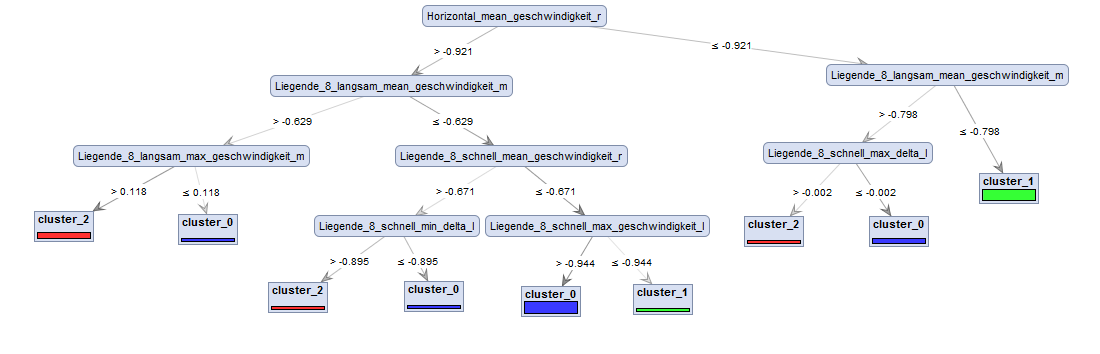
\includegraphics[width=15cm]{pics/EntscheidungsbaumCluster.PNG}
		\par\end{centering}
	\caption{\label{fig:EntscheidungsBaum}Entscheidungsbaum}
\end{figure}
Nach ein paar Stichproben k\"onnte man sagen, dass die Versuchspersonen, die im Cluster 1 sind, die mit den besten Ergebnissen sind, was das Verfolgen der Punkte angeht. In Cluster 2 sind die Versuchspersonen, bei denen gr\"o"stenteils nicht zu erkennen ist, welcher Versuch durchgef\"uhrt wurde und wo viele Fehlwerte drin sind. In Cluster 0 sind die Versuchspersonen gelandet, die im Mittelfeld sind. Die Stichproben wurden mittels Vergleich mit den Visualisierungen durchgef\"uhrt.

Das die Geschwindigkeit eine entscheidende Rolle spielt, ist dadurch erkl\"arbar, dass man wenn man die Versuche korrekt durchf\"uhrt keine gro"se Geschwindigkeit braucht. Schnelle Augenbewegungen weisen darauf hin, dass man seinen Blick korrigieren muss, um dem Targetpunkt wieder zu folgen, oder dass man sich nicht auf den Punkt konzentriert.